% move all configuration stuff into one file so we can focus on the content
\documentclass[aspectratio=169,hyperref={pdfpagelabels=false,colorlinks=true,linkcolor=white,urlcolor=lightblue},xcolor={table},t]{beamer}

%%%%%%%%%%%%%%%%%%%%%%%%%%%%%%%%%%%%%%%%%%%%%%%%%%%%%%%%%%%%%%%%%%%%%%%%%%%%%%%%%%
%%%%%%%%%%%%%%%%%%%%%%%%%%%%%%%%%%%%%%%%%%%%%%%%%%%%%%%%%%%%%%%%%%%%%%%%%%%%%%%%%%
% packages
\usepackage{pict2e}
\usepackage{epic}
\usepackage{amsmath,amsfonts,amssymb}
\usepackage{units}
\usepackage{fancybox}
\usepackage[absolute,overlay]{textpos} 
%\usepackage[table]{xcolor}
\usepackage{animate}
\usepackage{gensymb}
%\usepackage{graphicx}
%\usepackage{longtable}
\usepackage{multirow}
\usepackage{silence}
\usepackage{tikz}
\usepackage[backend=bibtex,style=ieee]{biblatex}
\AtEveryCitekey{\iffootnote{\tiny}{}}
%\addbibresource{include/references}



% fontsize
\let\Tiny=\tiny

%%%%%%%%%%%%%%%%%%%%%%%%%%%%%%%%%%%%%%%%%%%%%%%%%%%%%%%%%%%%%%%%%%%%%%%%%%%%%%%%%%
%%%%%%%%%%%%%%%%%%%%%%%%%%%%%%%%%%%%%%%%%%%%%%%%%%%%%%%%%%%%%%%%%%%%%%%%%%%%%%%%%%
% warnings
\pdfsuppresswarningpagegroup=1
\WarningFilter{biblatex}{Patching footnotes failed}
\WarningFilter{latexfont}{Font shape}
\WarningFilter{latexfont}{Some font shapes}
\WarningFilter{gensymb}{Not defining}


%%%%%%%%%%%%%%%%%%%%%%%%%%%%%%%%%%%%%%%%%%%%%%%%%%%%%%%%%%%%%%%%%%%%%%%%%%%%%%%%%%
%%%%%%%%%%%%%%%%%%%%%%%%%%%%%%%%%%%%%%%%%%%%%%%%%%%%%%%%%%%%%%%%%%%%%%%%%%%%%%%%%%
% theme & layout
\usetheme{Frankfurt}
\useinnertheme{rectangles}


%%%%%%%%%%%%%%%%%%%%%%%%%%%%%%%%%%%%%%%%%%%%%%%%%%%%%%%%%%%%%%%%%%%%%%%%%%%%%%%%%%
\setbeamertemplate{frametitle}[default][colsep=-4bp,rounded=false,shadow=false]
\setbeamertemplate{frametitle}
{%
    \nointerlineskip%
    %\vskip-0.5ex
    \begin{beamercolorbox}[wd=\paperwidth,ht=3.5ex,dp=0.6ex]{frametitle}
        \hspace*{1.3ex}\insertframetitle%
        
        \hspace*{1.3ex}\small\insertframesubtitle%
    \end{beamercolorbox}%
    \begin{textblock*}{100mm}(13.75cm,1cm)
        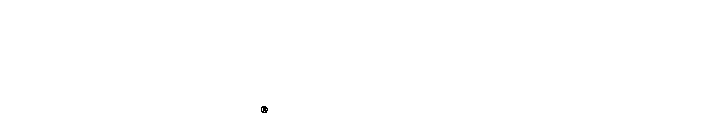
\includegraphics[height=.4cm,keepaspectratio]{../shared/Logo_GTCMT_white}
    \end{textblock*}
}


%%%%%%%%%%%%%%%%%%%%%%%%%%%%%%%%%%%%%%%%%%%%%%%%%%%%%%%%%%%%%%%%%%%%%%%%%%%%%%%%%%
\setbeamertemplate{title page}[default][colsep=-4bp,rounded=false,shadow=false]
\setbeamertemplate{title page}
{
    %\begin{textblock*}{100mm}(15cm,.51cm)
            %\href{https://github.com/alexanderlerch/ACA-Slides/blob/2nd_edition/\jobname.pdf}{\includegraphics[height=.5cm,keepaspectratio]{graph/Logo_github}}\hspace*{2ex}
    %\end{textblock*}
    %\begin{textblock*}{100mm}(15cm,1.3cm)
            %\href{\IEEELink}{\includegraphics[height=.5cm,keepaspectratio]{graph/icon/book}}\hspace*{2ex}
    %\end{textblock*}
    \vskip-10ex
    \begin{beamercolorbox}[wd=\paperwidth,ht=.7\paperheight,dp=0.6ex]{frametitle} %35ex
        %\begin{flushright}
            %\href{http://www.gtcmt.gatech.edu}{
\includegraphics[height=.8cm,keepaspectratio]{graph/Logo_GTCMT_black}}\hspace*{2ex}
        %\end{flushright}
        
        \hspace*{1.8ex}\LARGE\inserttitle%
        
        \vspace*{.5ex}
        
        \hspace*{1.3ex}\small\insertsubtitle%
        
        \vspace*{.5ex}
    \end{beamercolorbox}%
    \nointerlineskip%
    \begin{beamercolorbox}[wd=\paperwidth,ht=.4\paperheight,dp=0.6ex]{page number in head/foot}
        %\vspace*{-.5ex}
        \hspace*{1.7ex}\small\insertauthor%
        
        %\hspace*{1.7ex}\small }%
        
        \vspace*{12ex}
        \vfill
        \begin{flushright}
            \href{http://www.gtcmt.gatech.edu}{
\includegraphics[height=.5cm,keepaspectratio]{../shared/Logo_GTCMT_black}}\hspace*{2ex}
        \end{flushright}
    \end{beamercolorbox}%
}


%%%%%%%%%%%%%%%%%%%%%%%%%%%%%%%%%%%%%%%%%%%%%%%%%%%%%%%%%%%%%%%%%%%%%%%%%%%%%%%%%%
%\makeatother
\setbeamertemplate{footline}
{
  \leavevmode%
  \hbox{%
  \begin{beamercolorbox}[wd=.5\paperwidth,ht=2.25ex,dp=1ex,left,leftskip=1ex]{page number in head/foot}%
    \insertsubtitle
  \end{beamercolorbox}%
  \begin{beamercolorbox}[wd=.5\paperwidth,ht=2.25ex,dp=1ex,right,rightskip=1ex]{page number in head/foot}%
    \hfill
    \insertframenumber{} / \inserttotalframenumber
  \end{beamercolorbox}}%
  \vskip0pt%
}
%\makeatletter


%%%%%%%%%%%%%%%%%%%%%%%%%%%%%%%%%%%%%%%%%%%%%%%%%%%%%%%%%%%%%%%%%%%%%%%%%%%%%%%%%%
\beamertemplatenavigationsymbolsempty
\setbeamertemplate{navigation symbols}{}
\setbeamertemplate{blocks}[default]%[rounded=false,shadow=false]
\setbeamertemplate{itemize item}[square]
\setbeamertemplate{itemize subitem}[circle]
\setbeamertemplate{itemize subsubitem}[triangle]
\setbeamertemplate{enumerate item}[square]
\setbeamertemplate{enumerate subitem}[circle]
\setbeamertemplate{enumerate subsubitem}[circle]


%%%%%%%%%%%%%%%%%%%%%%%%%%%%%%%%%%%%%%%%%%%%%%%%%%%%%%%%%%%%%%%%%%%%%%%%%%%%%%%%%%
% colors
\setbeamercolor{structure}{fg=darkgray}
\setbeamercovered{transparent} %invisible
\setbeamercolor{bibliography entry author}{fg=black}
\setbeamercolor*{bibliography entry title}{fg=black}
\setbeamercolor*{bibliography entry note}{fg=black}
\setbeamercolor{frametitle}{fg=black}
\setbeamercolor{title}{fg=white}
\setbeamercolor{subtitle}{fg=white}
\setbeamercolor{frametitle}{fg=white}
\setbeamercolor{framesubtitle}{fg=white}
\setbeamercolor{mini frame}{fg=white, bg=black}
\setbeamercolor{section in head/foot}{fg=white, bg=darkgray}
\setbeamercolor{page number in head/foot}{fg=black, bg=gtgold}
\setbeamercolor{item projected}{fg=white, bg=black}

%---------------------------------------------------------------------------------

%%%%%%%%%%%%%%%%%%%%%%%%%%%%%%%%%%%%%%%%%%%%%%%%%%%%%%%%%%%%%%%%%%%%%%%%%%%%%%%%%%
%%%%%%%%%%%%%%%%%%%%%%%%%%%%%%%%%%%%%%%%%%%%%%%%%%%%%%%%%%%%%%%%%%%%%%%%%%%%%%%%%%
% title information
\title[]{MUSI6202: Digital Signal Processing for Music}   
\author[alexander lerch]{alexander lerch} 
%\institute{~}
%\date[Alexander Lerch]{}
%\titlegraphic{\vspace{-16mm}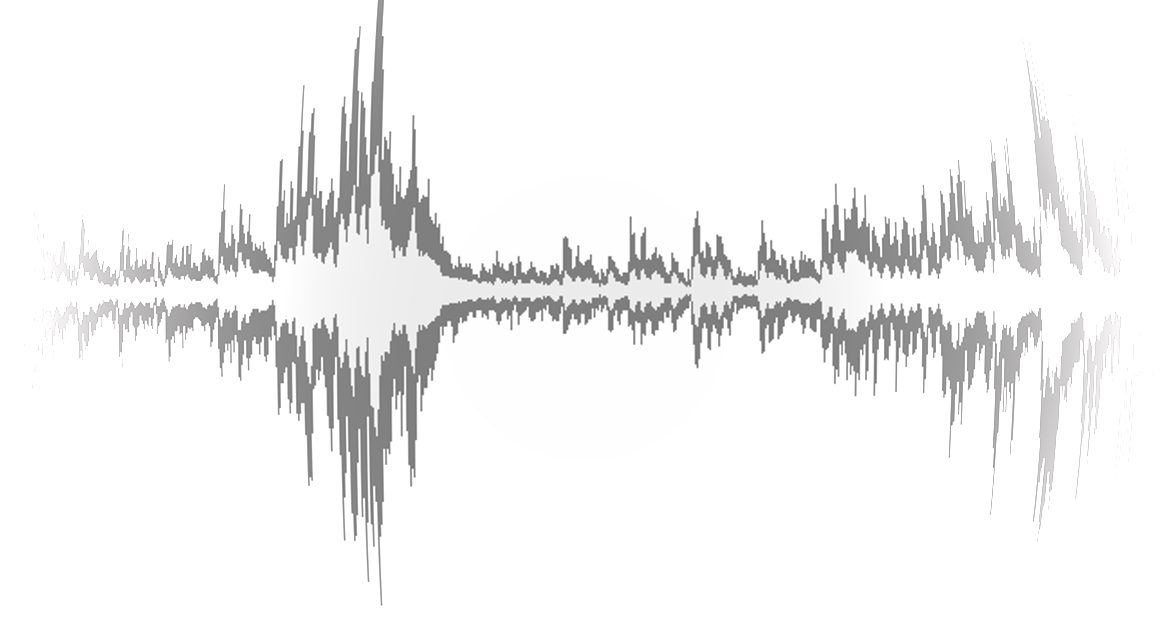
\includegraphics[width=\textwidth,height=3cm]{title}}

%%%%%%%%%%%%%%%%%%%%%%%%%%%%%%%%%%%%%%%%%%%%%%%%%%%%%%%%%%%%%%%%%%%%%%%%%%%%%%%%%%
%%%%%%%%%%%%%%%%%%%%%%%%%%%%%%%%%%%%%%%%%%%%%%%%%%%%%%%%%%%%%%%%%%%%%%%%%%%%%%%%%%
% colors
\definecolor{gtgold}{rgb}{.914, .664, 0} %0e7eed {rgb}{0.88,0.66,1,0.06} [234, 170, 0]/256 %96caff
\definecolor{darkgray}{rgb}{.15, .15, .15}
\definecolor{lightblue}{HTML}{0e7eed}
\definecolor{highlight}{rgb}{0, 0, 1} %_less!40

%%%%%%%%%%%%%%%%%%%%%%%%%%%%%%%%%%%%%%%%%%%%%%%%%%%%%%%%%%%%%%%%%%%%%%%%%%%%%%%%%%
%%%%%%%%%%%%%%%%%%%%%%%%%%%%%%%%%%%%%%%%%%%%%%%%%%%%%%%%%%%%%%%%%%%%%%%%%%%%%%%%%%
% relative paths
\graphicspath{{../graph/}}


%%%%%%%%%%%%%%%%%%%%%%%%%%%%%%%%%%%%%%%%%%%%%%%%%%%%%%%%%%%%%%%%%%%%%%%%%%%%%%%%%%
%%%%%%%%%%%%%%%%%%%%%%%%%%%%%%%%%%%%%%%%%%%%%%%%%%%%%%%%%%%%%%%%%%%%%%%%%%%%%%%%%%
% units
\setlength{\unitlength}{1mm}

%%%%%%%%%%%%%%%%%%%%%%%%%%%%%%%%%%%%%%%%%%%%%%%%%%%%%%%%%%%%%%%%%%%%%%%%%%%%%%%%%%
%%%%%%%%%%%%%%%%%%%%%%%%%%%%%%%%%%%%%%%%%%%%%%%%%%%%%%%%%%%%%%%%%%%%%%%%%%%%%%%%%%
% math
\DeclareMathOperator*{\argmax}{argmax}
\DeclareMathOperator*{\argmin}{argmin}
\DeclareMathOperator*{\atan}{atan}
\DeclareMathOperator*{\arcsinh}{arcsinh}
\DeclareMathOperator*{\sign}{sign}
\DeclareMathOperator*{\tcdf}{tcdf}
\DeclareMathOperator*{\si}{sinc}
\DeclareMathOperator*{\princarg}{princarg}
\DeclareMathOperator*{\arccosh}{arccosh}
\DeclareMathOperator*{\hwr}{HWR}
\DeclareMathOperator*{\flip}{flip}
\DeclareMathOperator*{\sinc}{sinc}
\DeclareMathOperator*{\floor}{floor}
\newcommand{\e}{{e}}
\newcommand{\jom}{\mathrm{j}\omega}
\newcommand{\jOm}{\mathrm{j}\Omega}
\newcommand   {\mat}[1]    		{\boldsymbol{\uppercase{#1}}}		%bold
\renewcommand {\vec}[1]    		{\boldsymbol{\lowercase{#1}}}		%bold

%%%%%%%%%%%%%%%%%%%%%%%%%%%%%%%%%%%%%%%%%%%%%%%%%%%%%%%%%%%%%%%%%%%%%%%%%%%%%%%%%%
%%%%%%%%%%%%%%%%%%%%%%%%%%%%%%%%%%%%%%%%%%%%%%%%%%%%%%%%%%%%%%%%%%%%%%%%%%%%%%%%%%
% media9
\newcommand{\includeaudio}[1]{
\href{run:audio/#1.mp3}{
\includegraphics[width=5mm, height=5mm]{graph/SpeakerIcon}}}

\newcommand{\includeanimation}[4]{{\begin{center}
                        \animategraphics[autoplay,loop,scale=.7]{#4}{animation/#1-}{#2}{#3}        
                        \end{center}
                        \addreference{matlab source: \href{https://github.com/alexanderlerch/ACA-Plots/blob/master/matlab/animate#1.m}{matlab/animate#1.m}}}
                        \inserticon{video}}
                        
%%%%%%%%%%%%%%%%%%%%%%%%%%%%%%%%%%%%%%%%%%%%%%%%%%%%%%%%%%%%%%%%%%%%%%%%%%%%%%%%%%
%%%%%%%%%%%%%%%%%%%%%%%%%%%%%%%%%%%%%%%%%%%%%%%%%%%%%%%%%%%%%%%%%%%%%%%%%%%%%%%%%%
% other commands
\newcommand{\question}[1]{%\vspace{-4mm}
                          \setbeamercovered{invisible}
                          \begin{columns}[T]
                            \column{.9\textwidth}
                                \textbf{#1}
                            \column{.1\textwidth}
                                \vspace{-8mm}
                                \begin{flushright}
                                     
\includegraphics[width=.9\columnwidth]{graph/question_mark}
                                \end{flushright}
                                \vspace{6mm}
                          \end{columns}\pause\vspace{-12mm}}

\newcommand{\toremember}[1]{
                        \inserticon{lightbulb}
                        }

\newcommand{\matlabexercise}[1]{%\vspace{-4mm}
                          \setbeamercovered{invisible}
                          \begin{columns}[T]
                            \column{.8\textwidth}
                                \textbf{matlab exercise}: #1
                            \column{.2\textwidth}
                                \begin{flushright}
                                     \includegraphics[scale=.5]{graph/logo_matlab}
                                \end{flushright}
                                %\vspace{6mm}
                          \end{columns}}

\newcommand{\addreference}[1]{  
                  
                    \begin{textblock*}{\baselineskip }(.98\paperwidth,.5\textheight) %(1.15\textwidth,.4\textheight)
                         \begin{minipage}[b][.5\paperheight][b]{1cm}%
                            \vfill%
                             \rotatebox{90}{\tiny {#1}}
                        \end{minipage}
                   \end{textblock*}
                    }
                    
\newcommand{\figwithmatlab}[1]{
                    \begin{figure}
                        \centering
                        \includegraphics[scale=.7]{#1}
                        %\label{fig:#1}
                    \end{figure}
                    
                    \addreference{matlab source: \href{https://github.com/alexanderlerch/MUSI-6202/blob/main/matlab/plot#1.m}{plot#1.m}}}
\newcommand{\figwithref}[2]{
                    \begin{figure}
                        \centering
                        \includegraphics[scale=.7]{#1}
                        \label{fig:#1}
                    \end{figure}
                    
                    \addreference{#2}}  
                                    
\newcommand{\inserticon}[1]{
                    \begin{textblock*}{100mm}(14.5cm,7.5cm)
                        \includegraphics[height=.8cm,keepaspectratio]{graph/#1}
                    \end{textblock*}}            

%%%%%%%%%%%%%%%%%%%%%%%%%%%%%%%%%%%%%%%%%%%%%%%%%%%%%%%%%%%%%%%%%%%%%%%%%%%%%%%%%%
%%%%%%%%%%%%%%%%%%%%%%%%%%%%%%%%%%%%%%%%%%%%%%%%%%%%%%%%%%%%%%%%%%%%%%%%%%%%%%%%%%
% counters
\newcounter{i}
\newcounter{j}
\newcounter{iXOffset}
\newcounter{iYOffset}
\newcounter{iXBlockSize}
\newcounter{iYBlockSize}
\newcounter{iYBlockSizeDiv2}
\newcounter{iXBlockSizeDiv2}
\newcounter{iDistance}

\newcommand{\IEEELink}{https://ieeexplore.ieee.org/servlet/opac?bknumber=9965970}

\addbibresource{../shared/references}



\subtitle{Part 7: Fourier Series}

%%%%%%%%%%%%%%%%%%%%%%%%%%%%%%%%%%%%%%%%%%%%%%%%%%%%%%%%%%%%%%%%%%%%%%%%%%%%
\begin{document}
    % generate title page
	\title[]{Digital Signal Processing for Music}   
\author[alexander lerch]{alexander lerch} 
%\institute{~}
%\date[Alexander Lerch]{}
\titlegraphic{\vspace{-16mm}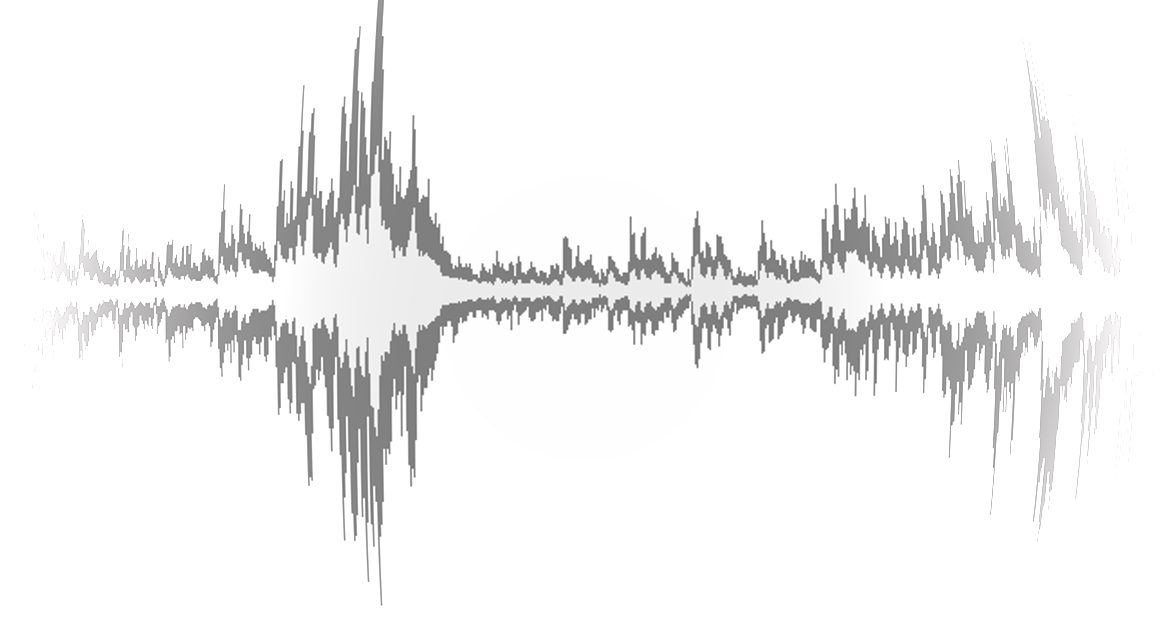
\includegraphics[width=\textwidth,height=3cm]{title}}


\begin{frame}
    \titlepage
    %\vspace{-5mm}
    \begin{flushright}
        \href{http://www.gtcmt.gatech.edu}{
\includegraphics[height=.8cm,keepaspectratio]{../shared/Logo_GTCMT_black}}
    \end{flushright}
\end{frame}


\section{introduction}
        \begin{frame}{Fourier analysis}{overview}
            \begin{enumerate}
                \item   \textbf{Fourier series}:\\ periodic signals as sum of sinusoidals
                \bigskip
                \item   \textbf{Fourier transform} (next slide deck):\\ frequency content of any signal
                    \begin{itemize}
                        \item   Fourier series to transform
                        \item   properties
                        \item   windowed Fourier transform
                    \end{itemize}
            \end{enumerate}
        \end{frame}

    \begin{frame}{Fourier series}{introduction}
        \begin{itemize}
            \item   periodic signals are \textbf{superposition of sinusoidals}
            \smallskip
            \item<2-> \textbf{properties}
                \begin{itemize}
                    \item   amplitude $a_k$
                    \item   frequency as integer multiple $k$ of fundamental $f_0$
                    \item   phase $\Phi_k$
                \end{itemize}
                \begin {equation*}
                    x(t) = \sum\limits_{k=0}^{\infty} a_k \sin(k\omega_0 t + \Phi_k) \nonumber
                \end {equation*}
            \smallskip
            \item<3->   \textbf{observations}
                \begin{itemize}
                    \item   time domain is continuous ($t$)
                    \item   frequency domain is discrete ($\sum$)
                \end{itemize}
        \end{itemize}
    \end{frame}

        \section{complex representation}
        \begin{frame}{Fourier series}{complex representation 1/2}
            \begin {equation*}
                x(t) = \sum\limits_{k=0}^{\infty} a_k \sin(k\omega_0 t + \Phi_k) \nonumber
            \end {equation*}
            \pause
            \begin{itemize}
                \item   trigonometric identity $\sin(a+b) = \sin(a)\cos(b) + \cos(a)\sin(b)$
                \item[$\Rightarrow$]
                \only<2>{
                \begin{equation*}
                    x(t) = \sum\limits_{k=0}^{\infty} {a_k \sin(\Phi_k)}\cdot\cos(k\omega_0 t) + {a_k \cos(\Phi_k)}\cdot\sin(k\omega_0 t)\nonumber
                \end{equation*}
                }
                \only<3->{
                \begin{equation*}
                    x(t) = \sum\limits_{k=0}^{\infty} \underbrace{a_k \sin(\Phi_k)}_{A_k}\cdot\cos(k\omega_0 t) + \underbrace{a_k \cos(\Phi_k)}_{B_k}\cdot\sin(k\omega_0 t)\nonumber
                \end{equation*}
                }
            \end{itemize}
        \end{frame}
        \begin{frame}{Fourier series}{complex representation 2/2}
            \begin{eqnarray*}
                e^{\mathrm{j}\omega t} &=& \cos(\omega t) + \mathrm{j}\sin(\omega t)\nonumber\\
                \mathrm{j} &=& \sqrt{-1}\nonumber
            \end{eqnarray*}

                \question{phasor representation in complex plane}
            \begin{eqnarray*}
                \cos(\omega t) &=& \only<2>{?}\only<3->{\frac{1}{2}\left(e^{\mathrm{j}\omega t} + e^{-\mathrm{j}\omega t}\right)}\nonumber\\
                \sin(\omega t) &=& \only<2>{?}\only<3->{\frac{1}{2\mathrm{j}}\left(e^{\mathrm{j}\omega t} - e^{-\mathrm{j}\omega t}\right)}\nonumber
            \end{eqnarray*}
        \end{frame}
        \begin{frame}{Fourier series}{phasor representation}
            \begin{columns}
            \column{.5\linewidth}
                \vspace{-10mm}
                \includeanimation
                    {Phasor}
                    {00}
                    {160}
                    {10}
            \column{.5\linewidth}
                \begin{itemize}
                    \item   phasor representation:
                        \begin{enumerate}
                            \item   sine value is defined by magnitude and phase
                            \item   decreasing the amplitude $\Rightarrow$ shorter vector
                            \item   increasing the frequency $\Rightarrow$ increasing speed
                        \end{enumerate}
                \end{itemize}
            \end{columns}
        \end{frame}
        
        \begin{frame}{fundamentals}{conjugate complex multiplication}
            \begin{figure}
                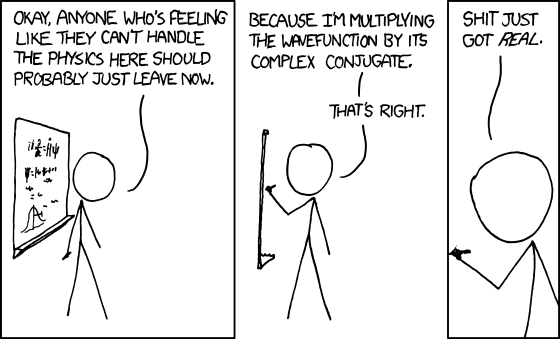
\includegraphics[scale=.45]{graph/xkcd_complex_conjugate}
            \end{figure}
            
            \addreference{\url{https://xkcd.com/849}}
        \end{frame}

        \begin{frame}{Fourier series}{real to complex}
            \vspace{-5mm}
            \begin{footnotesize}
            \begin{equation*}
                \cos(\omega t) = \frac{1}{2}\left(e^{\jom t} + e^{-\jom t}\right)\quad\quad
                \sin(\omega t) = \frac{1}{2\mathrm{j}}\left(e^{\jom t} - e^{-\jom t}\right)
            \end{equation*}
            %\begin{eqnarray*}
                %\cos(\omega t) &=& \frac{1}{2}\left(e^{\jom t} + e^{-\jom t}\right)\nonumber\\
                %\sin(\omega t) &=& \frac{1}{2\mathrm{j}}\left(e^{\jom t} - e^{-\jom t}\right)\nonumber
            %\end{eqnarray*}
            \pause
            \vspace{-2mm}
            \begin{eqnarray*}
                x(t) &=& \sum\limits_{k=0}^{\infty} A_k\cos(k\omega t) + B_k\sin(k\omega t)\nonumber\\
                &=& \sum\limits_{k=0}^{\infty} \frac{A_k}{2}\left(e^{\jom kt} + e^{-\jom kt}\right) - \mathrm{j}\frac{B_k}{2}\left(e^{\jom kt} - e^{-\jom kt}\right)\nonumber\\
                &=& \sum\limits_{k=0}^{\infty} \frac{1}{2}\left(A_k-\mathrm{j}B_k\right)e^{\jom kt} +  \frac{1}{2}\left(A_k+\mathrm{j}B_k\right)e^{-\jom kt}\nonumber\\
                &=& \sum\limits_{k=0}^{\infty} \underbrace{\frac{1}{2}\left(A_k-\mathrm{j}B_k\right)}_{c_k}e^{\jom kt} +  \frac{1}{2}\left(A_k+\mathrm{j}B_k\right)e^{-\jom kt}\nonumber
            \end{eqnarray*}
            \begin{equation*}\nonumber
               \text{with } c_{-k} := c^\ast_k \Rightarrow\;\; x(t) = \sum\limits_{k=-\infty}^{\infty} c_k e^{\jom_0kt}
            \end{equation*}
            \end{footnotesize}
        \end{frame}

    %\begin{frame}{Fourier series}{conjugate complex multiplication}
        %\begin{figure}
            %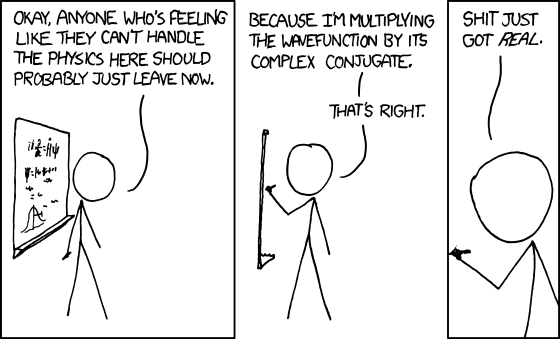
\includegraphics[scale=.45]{graph/xkcd_complex_conjugate}
        %\end{figure}
        %
        %from \url{https://xkcd.com/849}
    %\end{frame}

    \section{coefficients}
        \begin{frame}{Fourier series}{coefficients}
            \vspace{-5mm}
            \begin{footnotesize}
            \begin{equation*}\nonumber
               x(t) = \sum\limits_{k=-\infty}^{\infty} c_k e^{\jom_0kt}
            \end{equation*}
            \begin{enumerate}
                \item   multiply both sides with $e^{-\jom_0nt}$: $x(t)\cdot e^{-\jom_0nt} = \sum\limits_{k=-\infty}^{\infty} c_k e^{\jom_0(k-n)t}$
                    %\begin{equation*}\nonumber
                        %
                    %\end{equation*}
                \item   integrate both sides: $\int\limits_0^{T_0}{x(t)\cdot e^{-\jom_0nt}}dt = \int\limits_0^{T_0}\sum\limits_{k=-\infty}^{\infty} c_k e^{\jom_0(k-n)t}dt$
                    %\begin{equation*}\nonumber
                        %
                    %\end{equation*}
                \item   flip sum and integral: $ \int\limits_0^{T_0}{x(t)\cdot e^{-\jom_0nt}}dt = \sum\limits_{k=-\infty}^{\infty}c_k \int\limits_0^{T_0} e^{\jom_0(k-n)t}dt$
                    %\begin{equation*}\nonumber
                        %
                    %\end{equation*}
                \begin{eqnarray*}
                    \int\limits_0^{T_0} e^{\jom_0(k-n)t}dt &= 0 \;\;\;k\neq n\quad\quad\quad
                    \int\limits_0^{T_0} e^{\jom_0(k-n)t}dt &= T_0 \;\;\;k= n\nonumber\\
                    \Rightarrow &\int\limits_0^{T_0}{x(t)\cdot e^{-\jom_0nt}}dt = c_n T_0&
                \end{eqnarray*}
            \end{enumerate}
            \end{footnotesize}
        \end{frame}


    \begin{frame}{Fourier series}{limited number of coefficients}
        reconstruction of periodic signals with a limited number of sinusoidals:
        \begin {equation*}
            \hat{x}(t) = \sum\limits_{k=-\mathcal{K}}^{\mathcal{K}} c_k e^{\jom_0kt}
        \end {equation*}
        \only<1>{
        \figwithmatlab{FourierSeries}
        %\begin{figure}
            %\centering
                %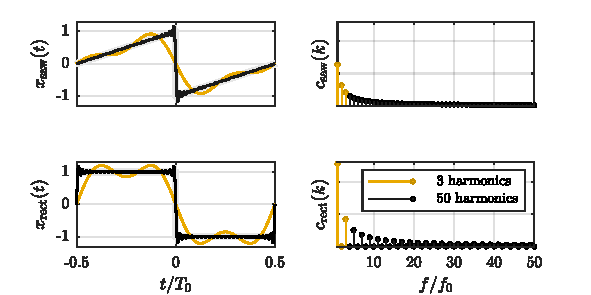
\includegraphics[width=\textwidth]{FourierSeries}
        %\end{figure}
        }
        \only<2>{
        \includeanimationnomatlab{FourierSeriesSquare/frame}{000}{059}{10}{\href{https://commons.wikimedia.org/wiki/File:Fourier_series_square_wave_circles_animation.gif}{commons.wikimedia.org/wiki/File:Fourier\_series\_square\_wave\_circles\_animation.gif}}{.5}
        }
        \only<3->{
        \includeanimationnomatlab{FourierSeriesSaw/frame}{000}{059}{10}{\href{https://commons.wikimedia.org/wiki/File:Fourier_series_square_wave_circles_animation.gif}{commons.wikimedia.org/wiki/File:Fourier\_series\_sawtooth\_wave\_circles\_animation.gif}}{.5}
        }
    \end{frame}

	
\section{summary}
    \begin{frame}{Fourier series}{summary 1/2}
        \begin{itemize}
            \item	any periodic signal $\Rightarrow$ representation in \textbf{Fourier Series}
                \only<1>{
                \begin {equation*}
                    x(t) = \sum\limits_{k=-\infty}^{\infty} c_k \e^{\mathrm{j}\omega_0 kt} \nonumber
                \end {equation*}}
                \only<2>{
                \begin {equation*}
                    x(t) = \sum\limits_{k=-\infty}^{\infty} c_k \e^{\mathrm{j}\textcolor{gtgold}{\omega_0} kt} \nonumber
                \end {equation*}}
                \only<3>{
                \begin {equation*}
                    x(t) = \sum\limits_{k=-\infty}^{\infty} c_k \textcolor{gtgold}{\e^{\mathrm{j}\omega_0 kt}} \nonumber
                \end {equation*}}
                \only<4>{
                \begin {equation*}
                    x(t) = \sum\limits_{k=-\infty}^{\infty} \textcolor{gtgold}{c_k} \e^{\mathrm{j}\omega_0 kt} \nonumber
                \end {equation*}}
                \only<5>{
                \begin {equation*}
                    x(t) = \sum\limits_{k=-\infty}^{\infty} c_k \e^{\mathrm{j}\omega_0 kt} \nonumber
                \end {equation*}}
                \pause
                \begin{itemize}
                    \item	$\omega_0 = 2\pi\cdot f_0$
                    \pause
                    \item	$\e^{\jom_0kt} = \cos(\omega_0kt) + \mathrm{j} \sin(\omega_0kt)$	\nonumber		
                \end{itemize}
        
            \pause
            \item	Fourier series coefficients $c_k$
                \begin {equation*}\label{eq:fourier_coeff}
                    c_k = \frac{1}{T_0}\int\limits_{-\nicefrac{T_0}{2}}^{\nicefrac{T_0}{2}} x(t) \e^{-\jom_0kt}\, dt \nonumber
                \end {equation*}
        \end{itemize}
    \end{frame}

    \begin{frame}{Fourier series}{summary 2/2}
        \begin{itemize}
            \item   complex coefficients are just a tool to represent the addition of sines neatly
            \smallskip
            \item<2->   to derive the coefficients from a signal we need
                \begin{itemize}
                    \item   fundamental frequency
                    \item   functional description
                \end{itemize}
            \smallskip
            \item<3->   ``frequency domain'' of Fourier series is discrete (integer multiples)
            \smallskip
            \item<4->   ``time domain'' can be continuous or discrete (discrete may be a pain to integrate, though)
        \end{itemize}
    \end{frame}
    
\end{document}

